%% CHAPTER 1

\section{General Situation Analysis}

	\subsection{Analysis of the Problem}
	
		The images are taken from a fixed camera. Making the difference between two
		frames is evident that camera has some little oscillations, but in general we
		could state a formal hypothesis of fixed camera, on which we will base all the
		analysis.
		
		There are some little problem that should be taken into account:
		\begin{itemize}
		  \item illumination may change during daytime, so the algorithm should be
		  robust against some of the derived problems, like shadows and reflections;
		  \item parallax is another problem with some relevance; over a certain angle
		  between camera axis and park spot, even the more robust algorithm will fail
		  because of the occlusions of the other parked cars.
		  \item there are some conclusions to derive for a bad parked car; if the car
		  occupy two parking spot, the algorithm must consider both spot busy, while if
		  one of the two park spot could be considered free, and another car may park,
		  the algorithm should report it as free;
		  \item occlusions: we have already touched this point, but some object may
		  occlude some parking spot, i.e. a street lamp between the camera and the
		  observed park spot.
		\end{itemize}
		
		For this problem we could derive some simple answer that generally speaking
		should be implemented:
		\begin{itemize}
		  \item The illumination problem could be bypassed using some different color
		  space, like the HSV and transforming the image in gray-scale.
		  \item The problem of the parallax make the use of rectangles to select a
		  park spot not a robust solution. When the parallax is to high, the only
		  feasible solution is to make use of another camera, because the problem will fall in a
		  problem of occlusion. If the parallax is not too high, the right answer is to
		  make use of a warping transformation, related to the four corner of the
		  single parking spot. This make the algorithm more robust also to the bad
		  parked car (see \ref{sub:warping}).
		  \item For small occlusions the only feasible solution is to create
		  different parameter for each park spot, that should be calibrated with
		  respect to its characteristics (occlusion as a characteristic). For very big
		  occlusions there is only one solution: change the camera's point of view.
		\end{itemize}
	
	\subsection{The Parking Spot}
	
		\subsubsection{The Parking Spot Object}
		
			The single parking spot object is initialized with a configuration file. The
			initialization follow this syntax:
			\begin{verbatim}
	%YAML:1.0
	parking_spot: 22
	spots: 
	[...]
	 - { nspot:2,  rect:[80,  427, 35, 37], 
	     polyx:[70,  118, 135,  93], 
	     polyy:[466, 465, 427, 424], 
	     param:[20000,30000,4,13,1] }
	[...]		
			\end{verbatim}
			where \verb+parking_spot+ is a global variable that will give the total number
			of parking spot that should be tracked, and \verb+spots+ is a list of
			associative arrays. In each associative array there are some variables that
			will be used in the code. The variable \verb+nspot+ is an id for the parking
			spot, \verb+rect+ is an array that represent a rectangle ($x$ top left
			position, $y$ top left position, width and height - this variable is
			currently unused). The variables \verb+ployx+ and \verb+polyy+ are two arrays
			that represent the four corner of a single parking spot. This point should be
			ordered, to create polylines. \verb+param+ is an ordered array of parameter
			used in different algorithms. 
			
			The \verb+ParkSpotObj+ is the class that represent a single parking spot,
			while the collection of the whole parking is a vector of object of that class.
			In the class, variables and methods are implemented to make the single park
			spot self-contained. Some algorithms implemented inside the object are:
			\begin{itemize}
			  \item initialization;
			  \item warping functions (see \ref{sub:warping});
			  \item some histograms operations, using the class \verb+Histogram+ that
			  implement some useful implementations to evaluate histograms component of
			  an image;
			  \item edge detection methods;
			  \item plotting and printing information on current frame or on
			  \verb+stdout+.
			\end{itemize}
		
		\subsubsection{The warping algorithm \label{sub:warping}}
		
		As we said before, to get as much information as possible we have to transform
		the quadrilateral parking spot (as perceived by the camera) in a rectangular
		image on which we could make some calculations.
		
		Given the four source corner $\mathbf{s_i}$ and the four destination corner
		$\mathbf{d_i}$, the transformation matrix is given by the solution of the
		equations:
		
		\begin{equation}
			\mathbf{d_i} - \mathbf{T}\times\mathbf{s_i} = 0 \qquad
			\mathrm{for}\,i=1,\ldots,4
		\end{equation}
		
		In particular, the code chose automatically the destination points on the
		basis of the bigger rectangle that contains the initial quadrilateral park
		spot. Once resolved $\mathbf{T}$, the transformation to extract the single,
		given a source matrix $\mathbf{S}$ and a destination matrix $\mathbf{D}$ is:
		
		\begin{equation}
			\mathbf{D}(x,y) = \mathbf{S}\left(
			\dfrac{T_{1,1}x+T_{1,2}y+T_{1,3}}{T_{3,1}x+T_{3,2}y+T_{3,3}},
			\dfrac{T_{2,1}x+T_{2,2}y+T_{2,3}}{T_{3,1}x+T_{3,2}y+T_{3,3}} \right)
		\end{equation}
		
		The optimization of this part of good is quite good. The transformation matrix
		is generated once, by the object constructor, while the transformation is
		called each frame by the \verb+ParkSpotObj::refreshImage()+ method (and
		similar).
		
		\begin{figure}[H] \label{fig:warping}
			\centering
				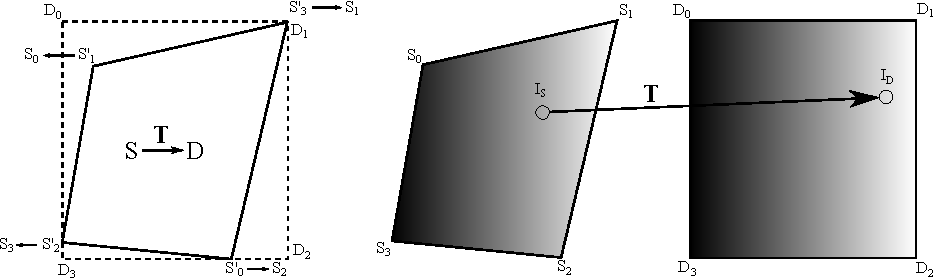
\includegraphics[keepaspectratio, scale=0.6]{img/warping.pdf}
			\caption{Representation of the warping algorithm}
		\end{figure}